\title{\fontsize{24}{28}\selectfont \textbf{Statistiche d'ordine dinamiche}}

\vspace{0.8cm}

\begin{tcolorbox}[colback=lightgray!20,colframe=black,arc=3mm, auto outer arc,]
                  
    \textbf{B: Statistiche d'ordine dinamiche}
    \begin{itemize}
    
    \item Vogliamo confrontare varie implementazioni di statistiche d’ordine dinamiche:
    
    \begin{enumerate}
        \item Con lista ordinata
        \item con ABR senza attributo size
        \item Come visto a lezione
    \end{enumerate}
    \item Per fare questo dovremo:
    
        \begin{itemize}
          
            \item Scrivere i programmi Python (no notebook) che:
          
            \begin{itemize}
            
                \item implementino quanto richiesto
                
                \item eseguono un insieme di test che ci permettano di comprendere vantaggi e svantaggi delle diverse implementazioni
                
            \end{itemize}
                
            \item Svolgere ed analizzare opportuni esperimenti

            \item Scrivere una relazione (in LaTeX) che descriva quanto fatto

            \item Nota: le strutture dati devono sempre essere implementate nel progetto; non si possono utilizzare librerie sviluppate da altri o copiare codice di altri

            
        \end{itemize}
        
    \end{itemize}
\end{tcolorbox}

\section{Spiegazione teorica dell'esercizio}
\subsection{Introduzione}
L'esercizio richiede di implementare le statistiche d'ordine dinamiche non solo nel classico metodo, ovvero con un albero rosso nero con in aggiunta l'attributo size, ma anche con un comune albero binario di ricerca e con una lista collegata da puntatori, in particolare che sia già ordinata (D'ora in avanti mi riferirò a questa struttura dati come lista ordinata). Fatto ciò, si vuole misurare la complessità computazionale delle operazioni tipiche delle statistiche d'ordine dinamiche, \textbf{Os-Rank} e \textbf{Os-Select}, su ciascuna delle tre implementazioni, al fine di decidere quale delle tre strutture dati convenga di più usare.

\subsection{Concetti teorici sulle strutture dati}
Per eseguire i test sopra citati avremo bisogno di sfruttare alcune operazioni di base come \textbf{inserimento} e \textbf{ricerca}, oltre appunto a \textbf{Os-Rank} e \textbf{Os-Select}. In questo paragrafo verrà fornita una breve spiegazione su come queste operazioni vengono implementate sulla struttura dati, insieme ad una descrizione sintetica sulle caratteristiche degli alberi e della lista. Cominciamo da quest'ultima.

\begin{itemize}
    \item \textbf{Albero binario di ricerca}: si tratta di una struttura dati, in particolare di un albero dove ogni nodo ha al massimo due figli. Esso viene costruito rispettando la seguente proprietà: chiave del figlio destro < chiave in cui mi trovo < chiave figlio sinistro. Per ogni albero devo disporre dei seguenti campi: un puntatore alla radice (il primo nodo), un puntatore al figlio sinistro, un puntatore al figlio destro, un puntatore a padre (Perciò il puntatore al padre della radice punterà a niente) ed infine la chiave del nodo, ovvero il valore che esso contiene.
    \item \textbf{Albero rosso nero}: Ha le stesse proprietà di un albero binario di ricerca, ma ogni nodo possiede un attributo booleano "color" che, se rispetta le seguenti proprietà, garantisce che non ci siano alberi degeneri (Un esempio di albero degenere può essere un albero con solo figli sinistri, che diventerebbe una lista puntata...)
    \begin{enumerate}
        \item Ogni nodo è rosso o nero
        \item La radice è nera
        \item Ogni foglia è nera
        \item Se un nodo è rosso, allora entrambi i suoi figli sono neri
        \item Tutti i camini da un nodo alle foglie contengono lo stesso numero di nodi neri
    \end{enumerate}
    \item \textbf{Lista ordinata}: Un semplice "elenco" di elementi sistemati in ordine crescente. Ogni nodo della lista è costituito dalla chiave e da un puntatore all'elemento successivo (Il puntatore a "next" dell'ultimo elemento punta a null)
\end{itemize}

\begin{figure}[h]
    \centering
    \begin{subfigure}[H]{0.4\textwidth}
        \centering
        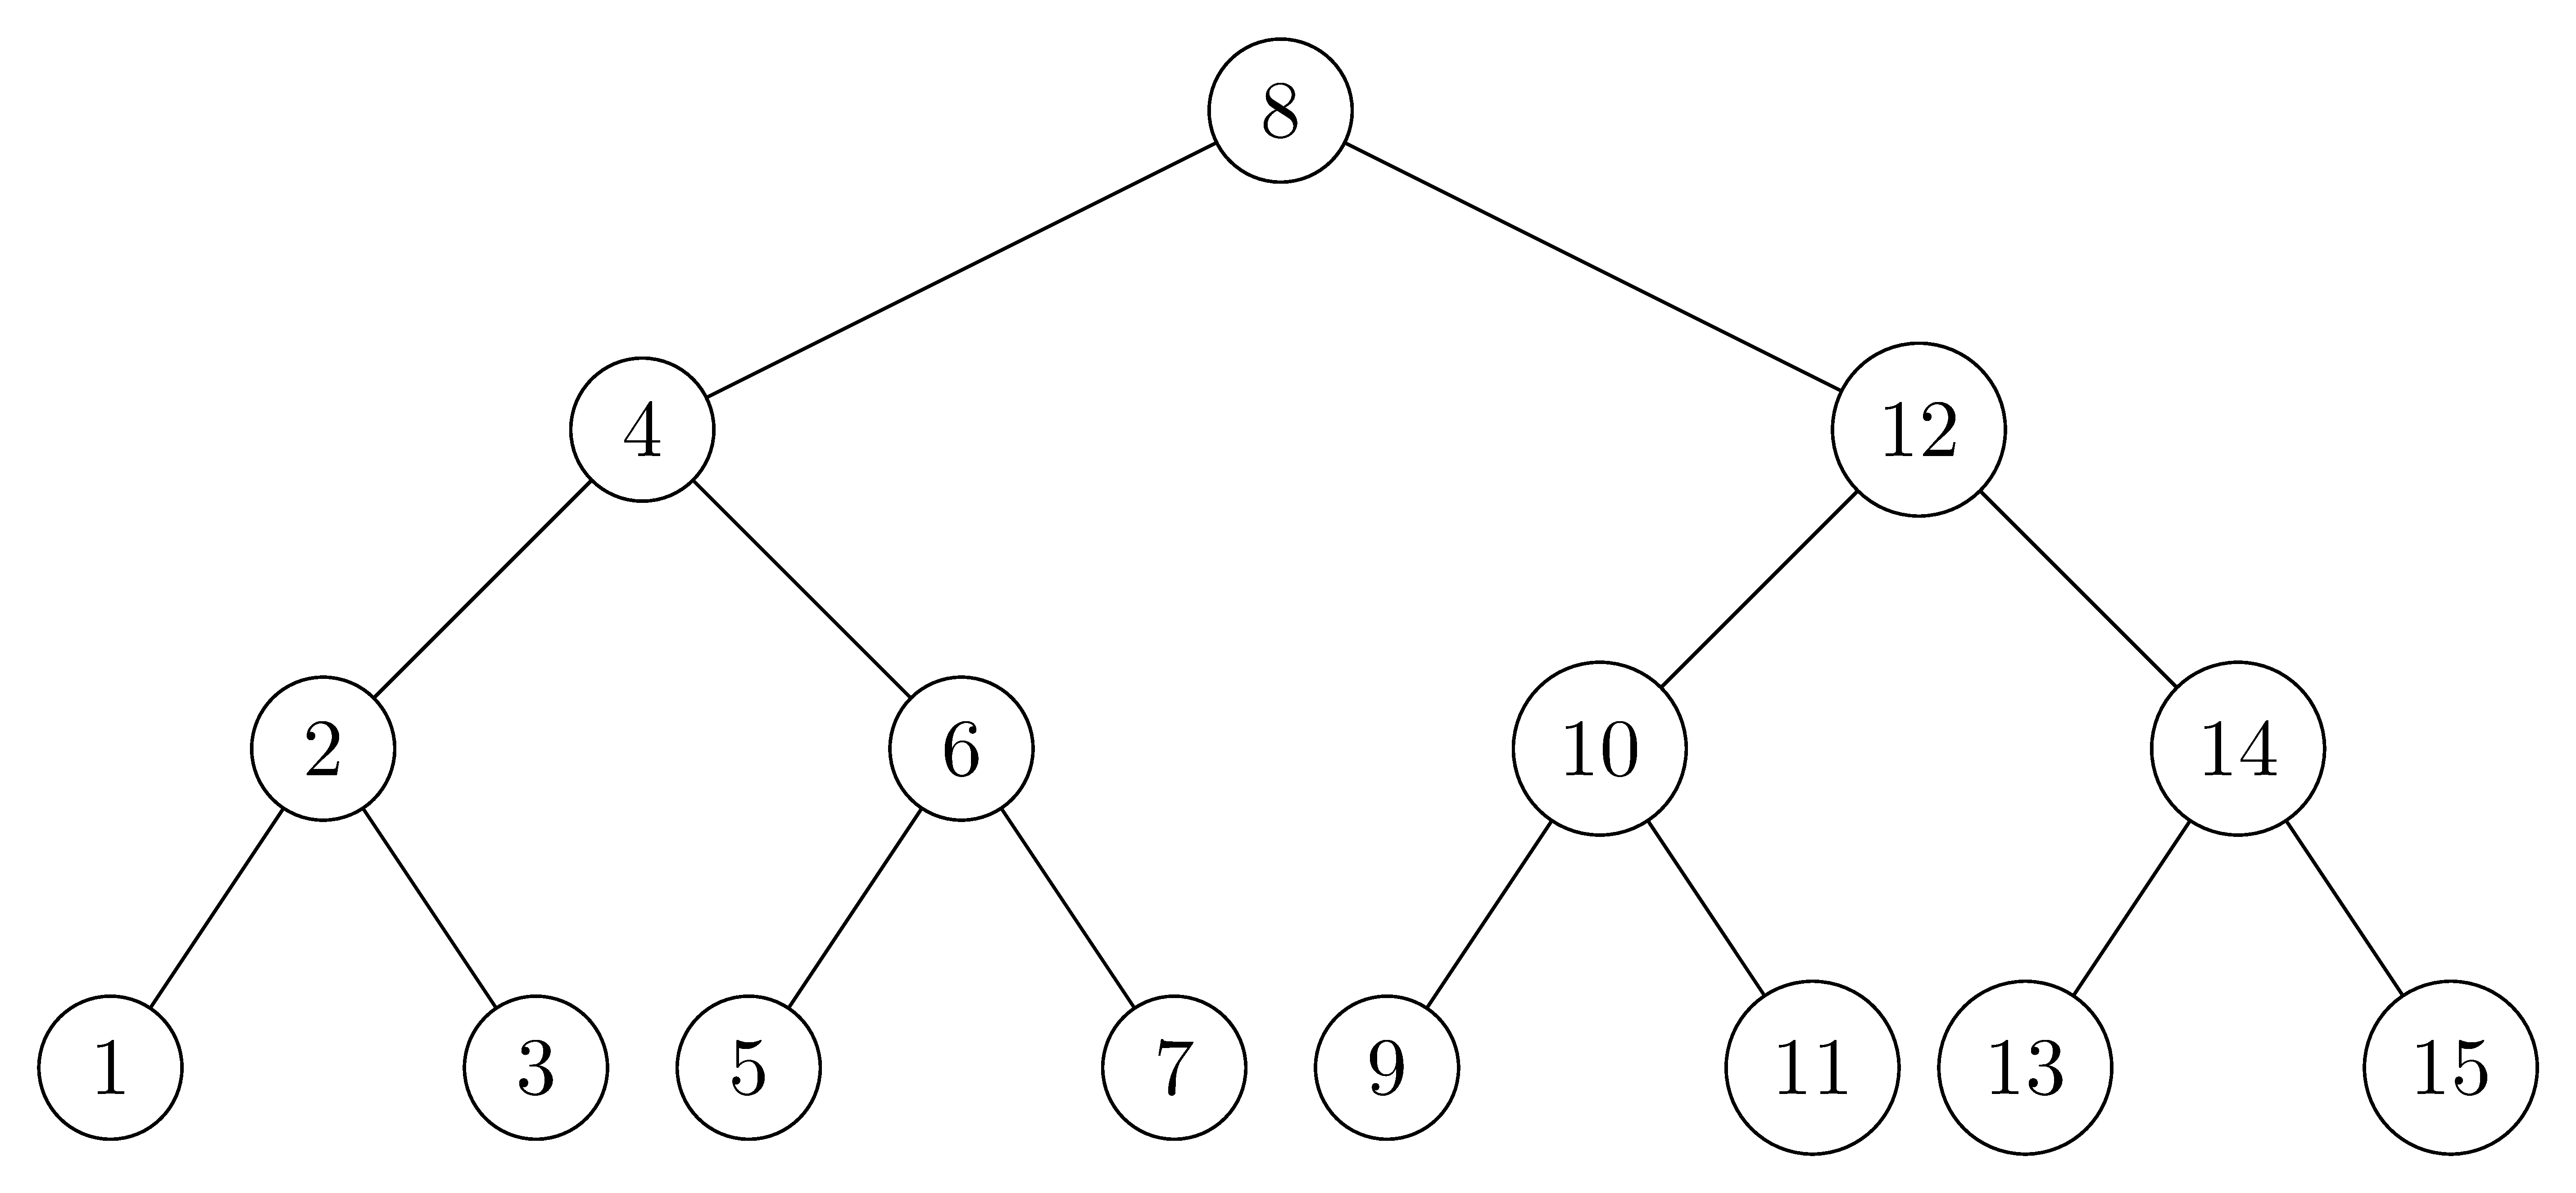
\includegraphics[width=1\textwidth]{Images/ABR.png}
        \caption{Albero binario di ricerca}
    \end{subfigure}
    \hfill
    \begin{subfigure}[H]{0.4\textwidth}
        \centering
        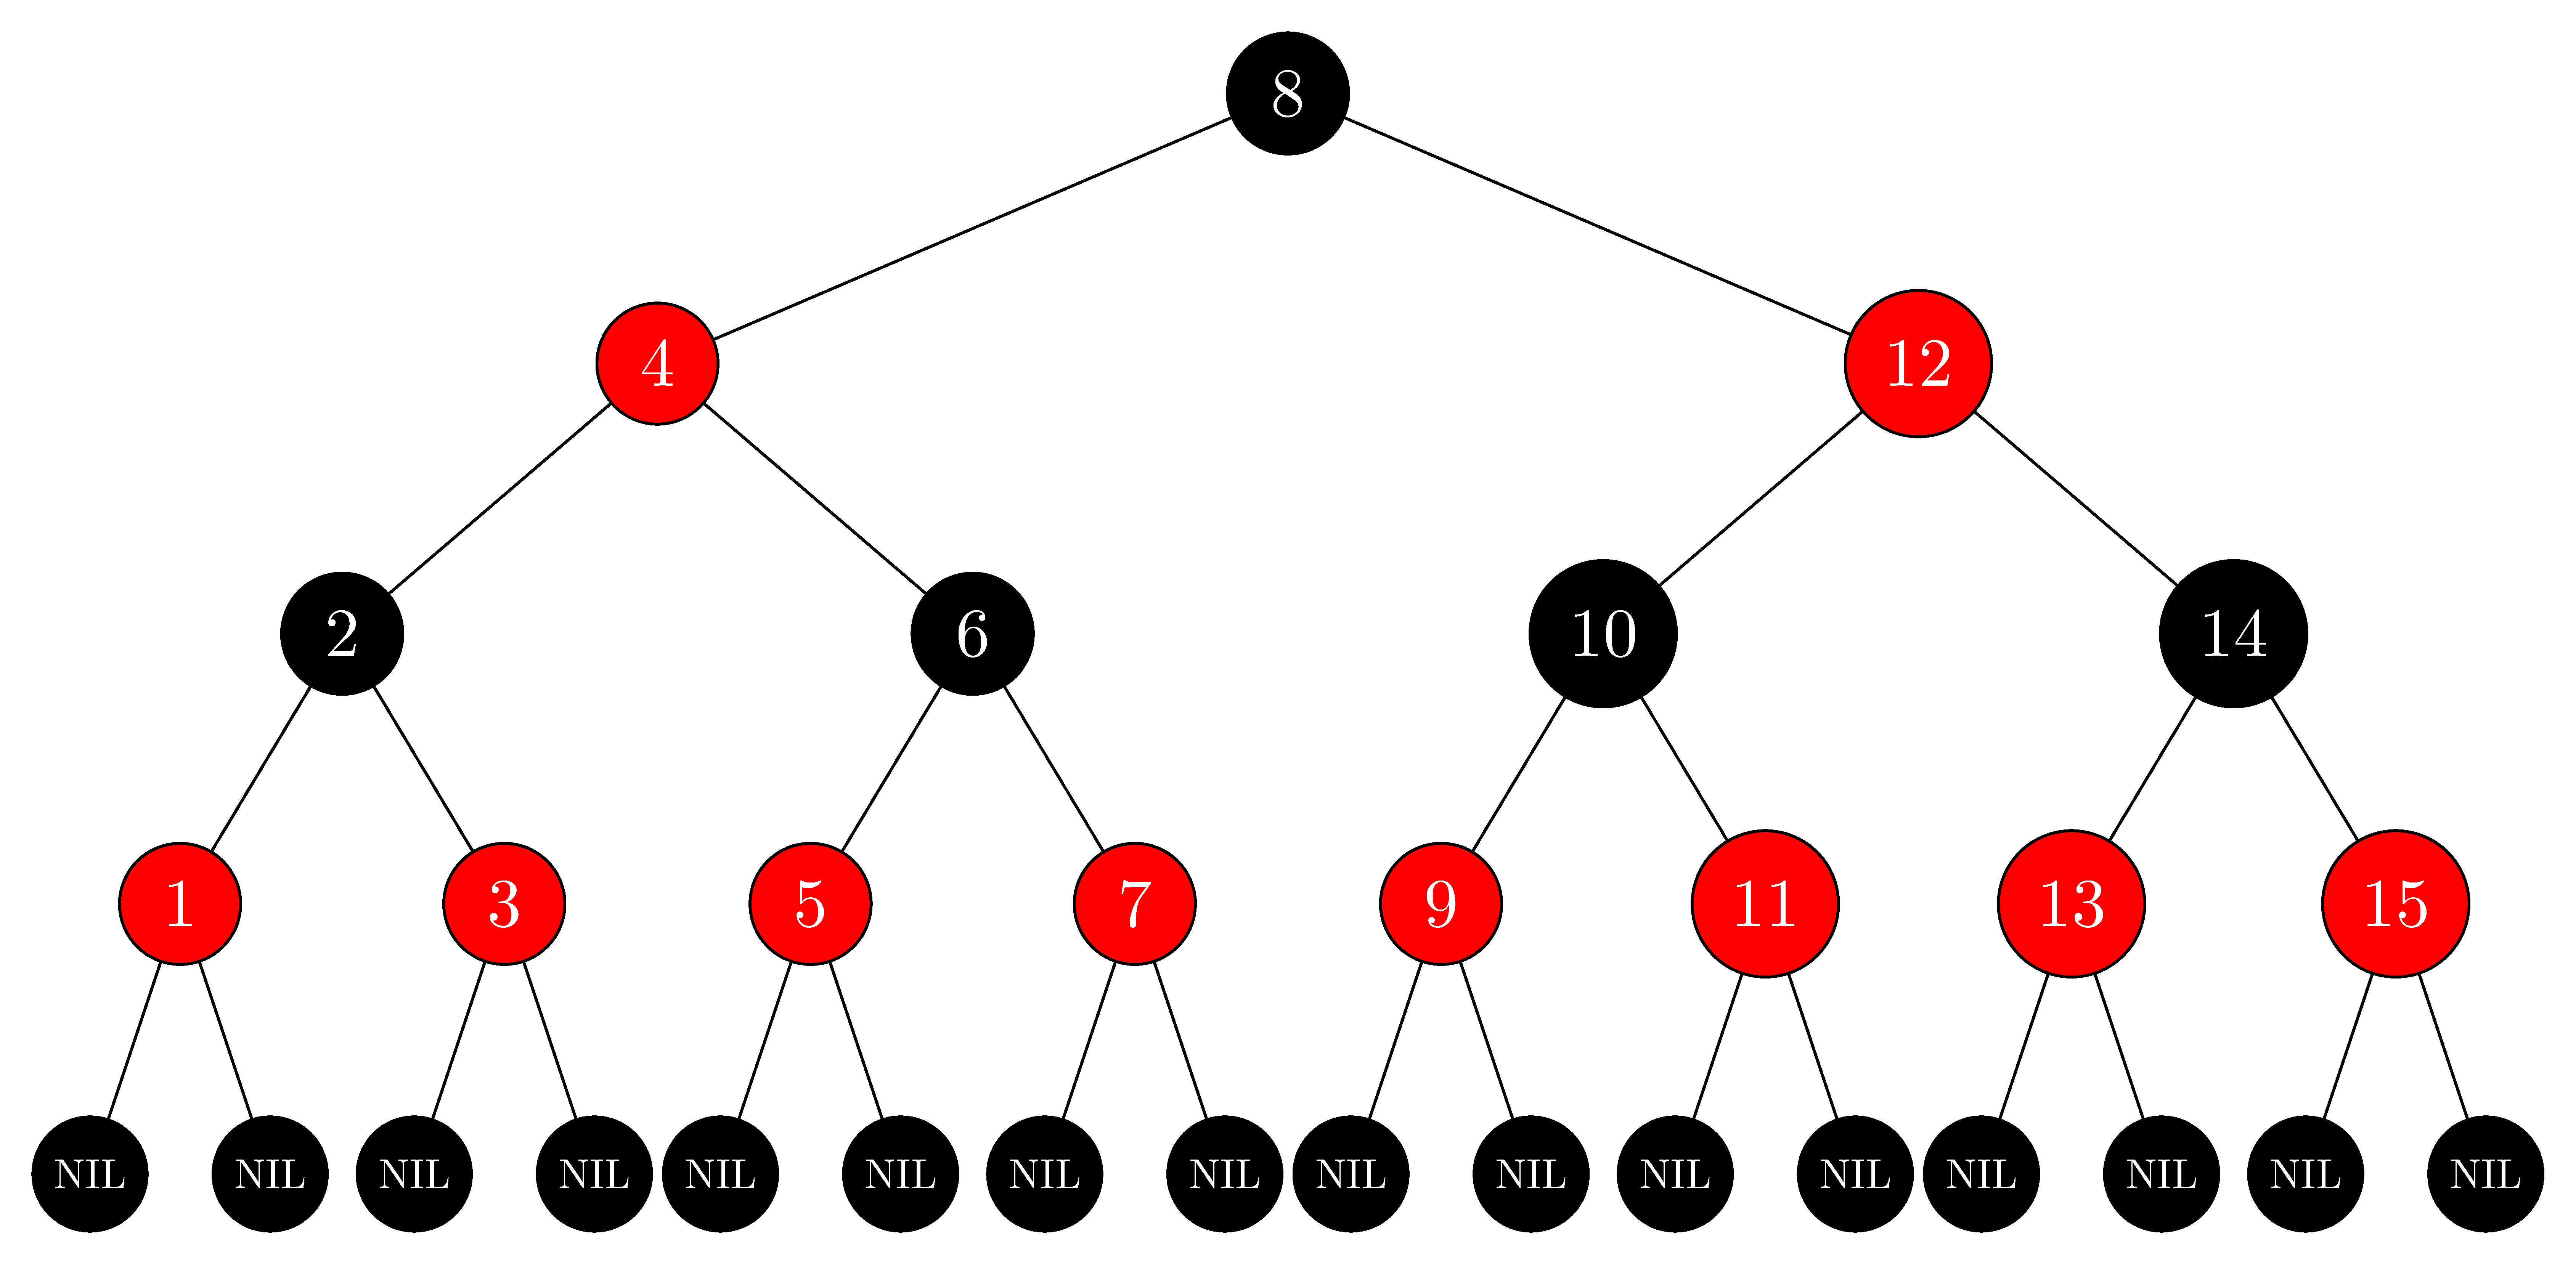
\includegraphics[width=1\textwidth]{Images/RB.png}
        \caption{Albero rosso nero}
    \end{subfigure}
    \hfill
    \begin{subfigure}[H]{0.6\textwidth}
        \centering
        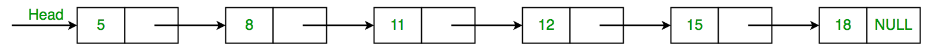
\includegraphics[width=1\textwidth]{Images/SL.png}
        \caption{Lista ordinata con puntatori}
    \end{subfigure}
    \caption{Tipologie di alberi}
\end{figure}

Adesso proseguiamo con la spiegazione di alcune operazioni utili che serviranno ai fini degli esperimenti

\begin{itemize}
\item Inserimento
    \begin{itemize}
        \item Albero Binario di Ricerca: Inizio dalla radice dell'albero ed imposto delle variabili che tengano traccia del nodo padre e del nodo figlio, quindi discendo lungo l'albero, spostandomi via via o a sinistra o a destra, a seconda se la chiave da inserire è rispettivamente minore o maggiore della corrente. Infine aggiusto i puntatori.
        \item Albero Rosso Nero: Il procedimento è il medesimo, con la differenza che il colore del nodo inserito viene impostato a "rosso" e che viene successivamente chiamata la funzione fixup al fine di preservare le proprietà dell'albero rosso nero.
        \item Lista Ordinata: Si inserisce l'elemento al posto corretto nella lista, spostando di un indice tutti gli elementi maggiori di quello nuovo ed aggiustando i puntatori.
    \end{itemize}
\item Ricerca
    \begin{itemize}
        \item Albero Binario di Ricerca: Mi muovo lungo l'albero con la stessa logica dell'inserimento e ad ogni nodo controllo che sia uguale a quello che sto cercando. In caso affermativo ritorno un puntatore al suddetto nodo, altrimenti, arrivati in fondo all'albero senza riscontrare successi, ritorno un puntatore vuoto.
        \item Albero Rosso Nero: Come sopra
        \item Lista Ordinata: L'algoritmo di ricerca binaria aiuta a trovare l'elemento richiesto senza bisogno di scorrere tutta la lista. Non avendone avuto bisogno ai fini dell'esperimento non è stato implementato nel codice e perciò non ci dilungheremo.
    \end{itemize}
\end{itemize}

Infine, le operazioni di cui vogliamo studiare la complessità

\begin{itemize}
\item Os-Rank
    \begin{itemize}
        \item Albero Binario di Ricerca: Si vuole il rango di un nodo con data chiave. Il rango è per definizione, il numero di elementi presenti nel sotto albero con radice in quel nodo più il nodo stesso. É stato pensato un tipo di approccio che sfrutta un'operazione molto comune, l'attraversamento \textbf{in order}. Nello specifico, per ogni nodo di cui vogliamo determinare il rango, si scorre l'albero fino a trovare il suddetto nodo, incrementando via via la variabile in cui si salva il rango.
        \item Albero Rosso Nero: Come sopra, con la differenza che, per definizione, le statistiche d'ordine dinamiche non sono altro che alberi rosso neri dove ad ogni nodo, oltre ai classici attributi left, right, parent e color si aggiunge anche size. Perciò non sarà necessario attraversare il sotto albero ad ogni iterazione per calcolarsi il rango, in quanto la dimensione sarà informazione fornita direttamente dal nodo che stiamo visitando.
        \item Lista Ordinata: Nel caso della lista, una volta fornito il nodo di cui si vuole il rango sarà necessario contare gli elementi uno ad uno scorrendola, nel caso peggiore, fino alla fine.
    \end{itemize}
\item Os-Select
    \begin{itemize}
        \item Albero Binario di Ricerca: Si vuole il puntatore al nodo che contiene l' n-esima chiave più piccola nel sotto albero con radice nel nodo dato. Come sopra, si dovrà scorrere tutto il sotto albero tramite l'attraversamento \textbf{in order}.
        \item Albero Rosso Nero: Il ragionamento è il medesimo; la size del nodo ci viene fornita dalla struttura dati stessa e perciò non va ricalcolata.
        \item Lista Ordinata: Come sopra.
    \end{itemize}
\end{itemize}

\vspace{0.8cm}

\subsection{Complessità d'ipotesi}
Per gli Alberi binari di ricerca le operazioni di inserimento richiedono un tempo di $O(h)$, dove h è l'altezza dell'albero ed è pari a log n nel caso migliore, ovvero quello di un albero bilanciato, mentre è pari a $O(n)$ nel caso peggiore, quello di un albero degenere (o catena lineare di elementi).
Lo stesso vale per l'albero rosso nero, con la differenza che non avremo mai il caso peggiore, proprio perchè per definizione deve rispettare le proprietà sopra elencate.
Nella lista invece, l'inserimento ha un caso ottimo di $O(1)$ se trovo immediatamente il punto in cui inserire l'elemento, in quel caso si tratta solo di aggiornare i puntatori. Nel caso peggiore, quando la lista deve essere attraversata quasi tutta per trovare il punto di inserimento, il tempo stimato è $O(n)$ dove n è il numero di elementi della lista.

Giunti a questo punto, sappiamo che il tempo stimato per le operazioni \textbf{Os-Select} e \textbf{Os-Rank} è $O(log n)$ per le statistiche d'ordine dinamiche implementate con alberi rosso neri, ma per le altre due implementazioni possiamo solamente fare una stima.

Nel caso dell'albero binario di ricerca, dovendo scorrere il sotto albero per ogni nodo, potrebbe essere necessario $O(n)$ nel caso peggiore (lista concatenata) per entrambe le operazioni.

Per la lista ordinata invece, sia per \textbf{Os-Rank} che per \textbf{Os-Select} potremmo avvicinarci a $O(n)$ nel caso peggiore, ovvero quello in cui dobbiamo scorrere tutta la lista di n elementi.

\begin{figure}[h]
    \centering
    \begin{tabular}{|c|c|c|c|c|}
        \hline
         & Inserimento & Ricerca & Os-rank & Os-Select\\
        \hline
        ABR & $O(h)$ & $O(h)$ & $O(n)$ & $O(n)$\\
        \hline
        RB & $O(h)$ & $O(h)$ & $O(log n)$ & $O(log n)$\\
        \hline
        Lista ordinata & $O(n)$ & $O(n)$ & $O(n)$ & $O(n)$\\
        \hline
    \end{tabular}
    \caption{Tabella riassuntiva delle complessità stimate}
\end{figure}



Come accennato in precedenza le statistiche d'ordine dinamiche nascono con la necessità di voler aggiungere informazioni ad una struttura dati nota preservando i tempi di computazione conosciuti. Per questo per aumentare le strutture dati normalmente si seguono queste poche e semplici regole.
\begin{enumerate}
    \item Scegliere una struttura dati sottostante (Alberi RN)
    \item Determinare informazioni aggiuntive da gestire (size del nodo)
    \item Verificare che si possano gestire le informazioni aggiuntive per le operazioni esistenti sulla struttura dati con analoghi tempi di esecuzione (tenere aggiornato size durante inserimenti e cancellazioni)
    \item Sviluppare nuove operazioni (OS-Select e OS-Rank)
\end{enumerate}

Per gestire size in inserimento in modo efficiente incremento size di ogni nodo visitato mentre scendo nell'albero; dopotutto il nuovo nodo sarà un discendente di ogni nodo già visitato. Nelle rotazioni (Nel fixup) basta aggiungere in fondo allo pseudo codice y.size ← x.size e x.size ← x.left.size + x.right.size + 1, spendendo solamente O(1) per aggiornarlo ad ogni rotazione.

\vspace{0.8cm}

\section{Descrizione dei metodi implementati}
Di seguito un diagramma UML allo scopo di mostrare com'è stato strutturato il codice. Tutte e tre le tipologie di nodi hanno una relazione di aggregazione con i rispettivi alberi. Vi è anche una relazione di aggregazione tra \textbf{RBNode} e \textbf{Node} con molteplicità 3, dato che entrambe hanno all'interno le istanze del nodo padre, del figlio destro e del figlio sinistro.


\begin{figure}[H]
    \centering
     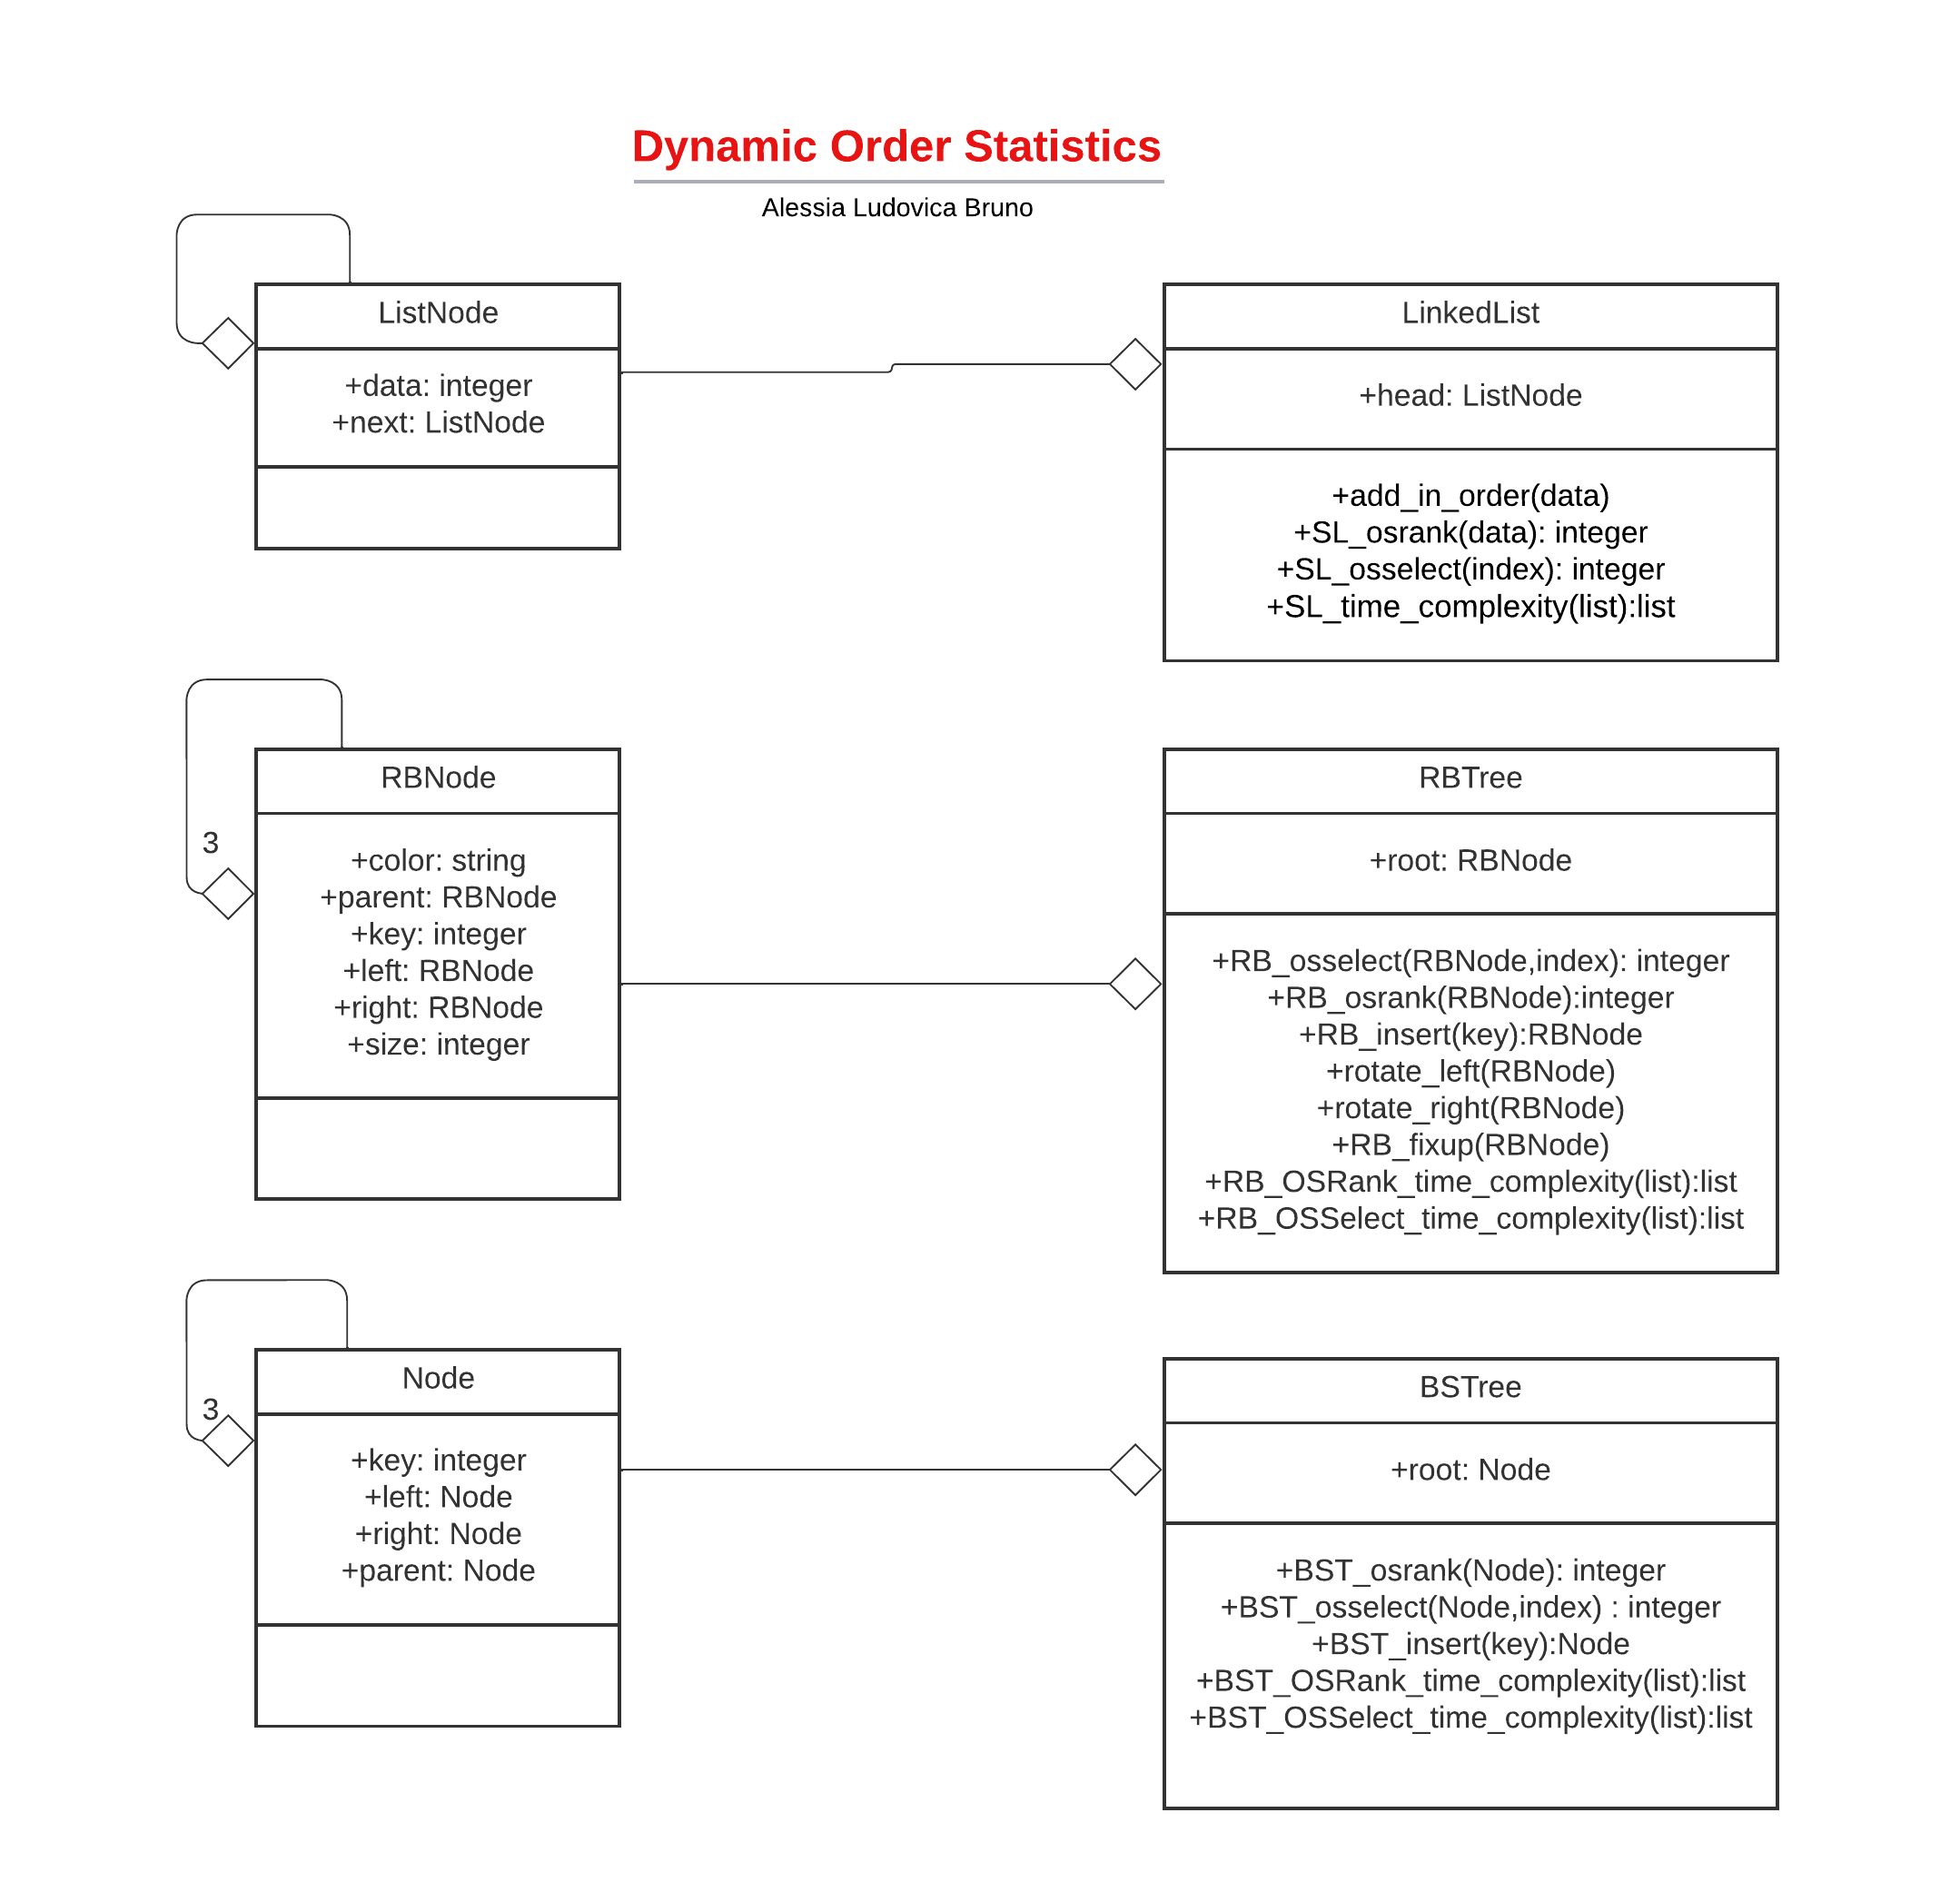
\includegraphics[width=1\textwidth]{Images/UML.png}
    \caption{UML realizzato con Lucidchart}
\end{figure}
Di seguito le funzionalità dei metodi divisi per struttura dati

\begin{itemize}
    \item \textbf{Lista ordinata}
    \begin{itemize}
    \item \textbf{add\_in\_order} inserisce l'elemento passato nella lista in modo da preservare l'ordine
    \item \textbf{SL\_osrank} Funzione os-rank implementata per la lista
    \item \textbf{SL\_osselect} Funzione os-select implementata per la lista
    \item \textbf{SL\_OSRank\_time\_complexity} Misura la complessità di os-rank per la lista ordinata, stampandone il grafico.
    \item \textbf{SL\_OSSelect\_time\_complexity} Misura la complessità di os-select per la lista ordinata, stampandone il grafico.
    \end{itemize}
    \item \textbf{Albero rosso nero}
    \begin{itemize}
        \item \textbf{RB\_insert} inserisce l'elemento passato nell'albero rosso nero
        \item \textbf{RB\_fixup} chiamato dall'inserimento per fare in modo che dopo l'aggiunta di un nuovo nodo vengano rispettate le proprietà dell'albero.
        \item \textbf{rotate\_left} rotazione per ribilanciare l'albero, metodo chiamato nel fixup.
        \item \textbf{rotate\_right} rotazione per ribilanciare l'albero, metodo chiamato nel fixup.
        \item \textbf{RB\_osrank} Funzione os-rank implementata per l'albero rosso nero
        \item \textbf{RB\_osselect} Funzione os-select implementata per l'albero rosso nero
        \item \textbf{RB\_OSRank\_time\_complexity}  Misura la complessità di os-rank per l'albero rosso nero, stampando il grafico.
        \item \textbf{RB\_OSSelect\_time\_complexity} Misura la complessità di os-select per l'albero rosso nero, stampando il grafico.  
    \end{itemize}
    
    \item \textbf{Albero binario di ricerca}
    \begin{itemize}
        \item \textbf{BST\_osselect} Funzione os-select implementata per l'albero binario di ricerca
        \item \textbf{BST\_osrank} Funzione os-rank implementata per l'albero binario di ricerca
        \item \textbf{BST\_insert} Inserisce il nodo passato nell'albero binario di ricerca
        \item \textbf{BST\_OSRank\_time\_complexity}  Misura la complessità di os-rank per l'albero binario di ricerca, stampando il grafico.
        \item \textbf{BST\_OSSelect\_time\_complexity} Misura la complessità di os-select per l'albero binario di ricerca, stampando il grafico.
    \end{itemize}
\end{itemize}

Infine abbiamo la funzione \textbf{search} che è fuori dalle classi perchè mi è utile per cercare i nodi in entrambe le tipologie di albero.

Il programma principale crea una lista di 2000 interi randomici compresi nell'intervallo tra 0 e 4000, passandoli alle funzioni incaricate di calcolare la complessità in modo tale da avere la stessa tipologia di elementi per ogni struttura dati. Inoltre ha il compito di creare dei grafici con gli elementi sopra citati e le liste dei tempi ritornate dalle funzioni in modo tale da confrontarli.


\section{Esperimenti}

\subsection{Descrizione degli esperimenti}
Per calcolare la complessità ci serviremo della libreria Python "matplotlib" che con la sua funzione plot(x,y) permette di creare grafici passandogli due liste di parametri.
Per tutte e tre le strutture dati la logica è stata la seguente: provare varie lunghezze di lista, da 10 fino a 2000 elementi, con un passo di dieci (Si provano quindi 200 lunghezze diverse di lista) e per ogni lunghezza salvare in un array il tempo necessario a svolgere la funzione richiesta. Viene fatta poi la media tra i tempi ottenuti, sommandoli e dividendoli per il numero di ripetizioni effettuato. Di seguito un pezzo di codice generico che mostra come sono strutturate le funzioni per calcolare a complessità.

\begin{figure}[H]
    \centering
     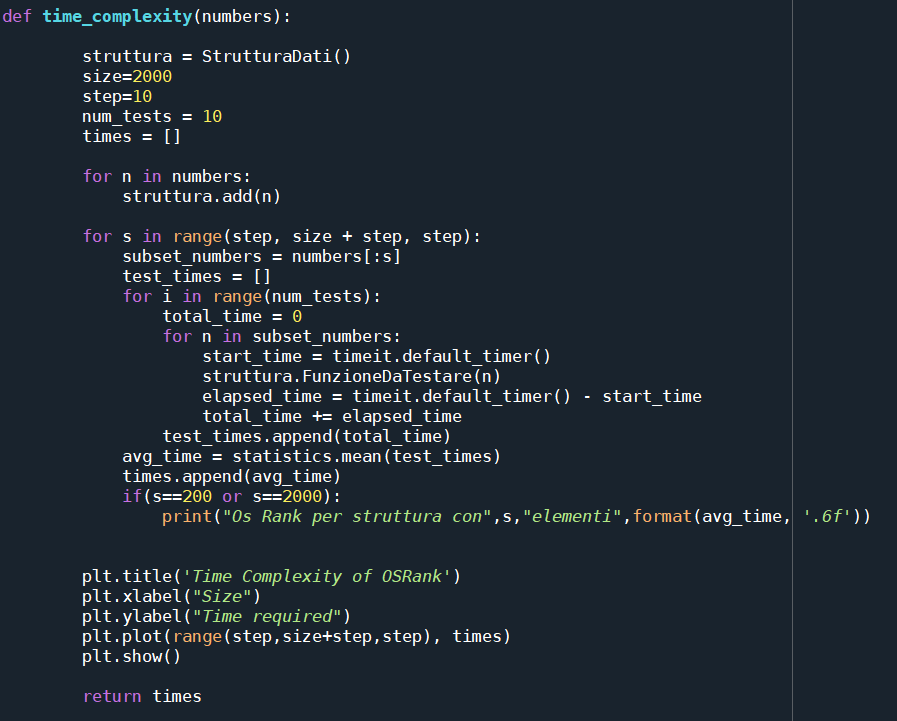
\includegraphics[width=1\textwidth]{Images/CODE_SAMPLE.png}
    \caption{Struttura generale delle funzioni}
\end{figure}

\subsection{Risultati sperimentali}
Di seguito verrà seguito lo stesso ordine usato nel codice
    \subsubsection{Lista ordinata}
    Come accennato, creo una lista chiamata "linked", imposto un range di lunghezze che va da 10 a 2000 con passo 10 (controllo quindi 200 liste diverse) e per ogni dimensione di lista, la riempio con elementi casuali e calcolo il rango per ognuno di questi, misurando il tempo di esecuzione. Per ottenere un grafico il più reciso possibile ho svolto i calcoli più di una volta tramite un apposito ciclo for e infine ho calcolato la media. Lo stesso vale per Os-select. Il risultato è stato il seguente

    \begin{figure}[h]
        \centering
        \begin{subfigure}[H]{0.4\textwidth}
            \centering
            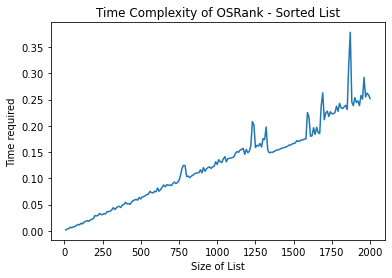
\includegraphics[width=1\textwidth]{Images/SL-RANK.png}
            \caption{Os-Rank}
        \end{subfigure}
        \begin{subfigure}[H]{0.4\textwidth}
            \centering
            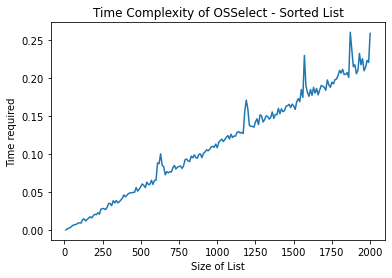
\includegraphics[width=1\textwidth]{Images/SL-SELECT.png}
            \caption{Os-Select}
        \end{subfigure}
    \caption{Complessità stimate sulla lista ordinata}
    \end{figure}

    Come premesso, la complessità di Os-rank ha chiaramente un andamento lineare $O(n)$, così come per Os-select.

    \vspace{1cm}
    
    \subsubsection{Albero rosso nero}
    Anche qui creo un albero, imposto la dimensione massima a 2000 elementi, il passo è sempre di 10, quindi anche qui controllo 200 alberi di dimensioni diverse. Uso la funzione search per cercare il nodo con la chiave scelta dall'algoritmo e restituirne il puntatore alla funzione rank. 
    Il ragionamento è stato il medesimo anche per select, con la differenza che ho dovuto aggiungere qualche linea di codice in più per scegliere un indice casuale "index" che rappresenterebbe la i-esima chiave più piccola che si sta cercando. Anche qui sono state fatte le medie dei grafici.
    Il risultato è stato il seguente:

    \begin{figure}[H]
        \centering
        \begin{subfigure}[H]{0.4\textwidth}
            \centering
            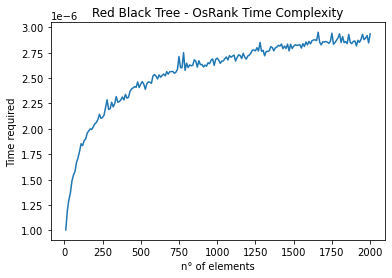
\includegraphics[width=1\textwidth]{Images/RB-RANK.png}
            \caption{Os-Rank}
        \end{subfigure}
        \begin{subfigure}[H]{0.4\textwidth}
            \centering
            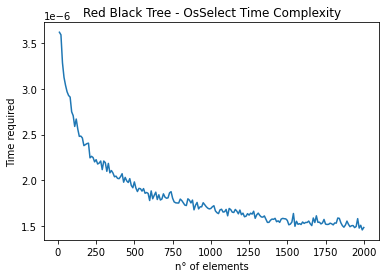
\includegraphics[width=1\textwidth]{Images/RB-SELECT.png}
            \caption{Os-Select}
        \end{subfigure}
    \caption{Complessità stimate sull'albero rosso nero (Struttura classica per le statistiche d'ordine dinamiche)}
    \end{figure}

    Dopo svariati tentativi si nota chiaramente che la complessità sarà sempre logaritmica, perciò si ha $O(log n)$ per entrambe le funzioni.
    Per Os-Select il grafico del logaritmo è in base minore di 2 probabilmente perchè os-select è stata implementata per scartare a priori dei nodi di cui la funzione search non riesce a trovare la chiave, restituendo quindi null.

    \subsubsection{Albero binario di ricerca}
    Il procedimento è il medesimo a sopra e l'andamento atteso è stato infatti lineare come per la lista ordinata, con una grossa differenza però nei tempi di esecuzione, come si può vedere dalla tabella a fine paragrafo. Qui non è stato necessario fare le medie.

    \begin{figure}[H]
        \centering
        \begin{subfigure}[H]{0.4\textwidth}
            \centering
            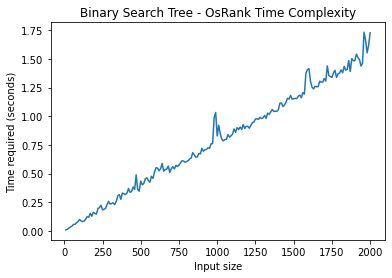
\includegraphics[width=1\textwidth]{Images/BST-RANK.png}
            \caption{Os-Rank}
        \end{subfigure}
        \begin{subfigure}[H]{0.4\textwidth}
            \centering
            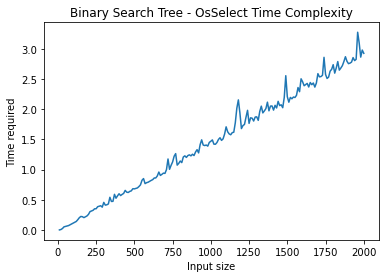
\includegraphics[width=1\textwidth]{Images/BST-SELECT.png}
            \caption{Os-Select}
        \end{subfigure}
    \caption{Complessità stimate sull'albero binario di ricerca}
    \end{figure}

    Abbiamo nuovamente un $O(n)$, ma con tempi decisamente maggiori a causa del dover scorrere l'albero ad ogni iterazione, operazione che viene ovviata nell'albero rosso nero, in quanto l'informazione è conservata nel nodo stesso, e nella lista ordinata. 

    \begin{figure}[h]
    \centering
    \begin{tabular}{|c|c|c|}
        \hline
         & Os-rank & Os-Select\\
        \hline
        SL 200 elementi & 0.024 & 0.020\\
        \hline
        SL 2000 elementi & 0.233 & 0.216\\
        \hline
        RN 200 elementi & 0.000002 & 0.000001\\
        \hline
        RN 2000 elementi & 0.000003 & 0.000002\\
        \hline
        ABR 200 elementi & 0.151 & 0.258\\
        \hline
        ABR 2000 elementi & 1.460 & 2.653\\
        \hline
    \end{tabular}
    \caption{Tabella riassuntiva dei tempi di esecuzione (in secondi)}
    \end{figure}

    \vspace{1cm}

    I grafici conclusivi riportati qui di seguito aiutano a visualizzare le differenze di andamento temporale riportate nella tabella.

    \begin{figure}[h]
    \centering
    \begin{subfigure}[H]{0.4\textwidth}
        \centering
        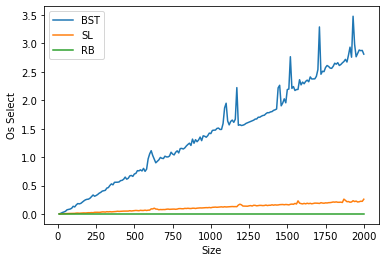
\includegraphics[width=1\textwidth]{Images/CONFRONTO-SELECT.png}
        \caption{OS-select}
    \end{subfigure}
    \hfill
    \begin{subfigure}[H]{0.4\textwidth}
        \centering
        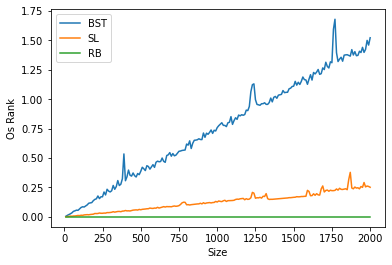
\includegraphics[width=1\textwidth]{Images/CONFRONTO-RANK.png}
        \caption{OS-rank}
    \end{subfigure}
    \caption{Confronto finale}
\end{figure}

\section{Conclusioni}

    A parità di tempi di inserimento e ricerca, per implementare le statistiche d'ordine dinamiche la struttura dati migliore è senza dubbio l'albero rosso nero, in quanto le sue proprietà gli impediscono di ricadere nel caso peggiore $O(n)$ e la corretta gestione dell'attributo size fa si che venga mantenuto un tempo logaritmico $O(logn)$. Se per qualsiasi motivo si decide di voler provare un'alternativa, tra albero binario di ricerca e lista ordinata si preferisce sicuramente la seconda, visti i tempi di esecuzione riportati dagli esperimenti.
